\documentclass[]{article}
\usepackage{lmodern}
\usepackage{amssymb,amsmath}
\usepackage{ifxetex,ifluatex}
\usepackage{fixltx2e} % provides \textsubscript
\ifnum 0\ifxetex 1\fi\ifluatex 1\fi=0 % if pdftex
  \usepackage[T1]{fontenc}
  \usepackage[utf8]{inputenc}
\else % if luatex or xelatex
  \ifxetex
    \usepackage{mathspec}
  \else
    \usepackage{fontspec}
  \fi
  \defaultfontfeatures{Ligatures=TeX,Scale=MatchLowercase}
\fi
% use upquote if available, for straight quotes in verbatim environments
\IfFileExists{upquote.sty}{\usepackage{upquote}}{}
% use microtype if available
\IfFileExists{microtype.sty}{%
\usepackage{microtype}
\UseMicrotypeSet[protrusion]{basicmath} % disable protrusion for tt fonts
}{}
\usepackage[margin=1in]{geometry}
\usepackage{hyperref}
\hypersetup{unicode=true,
            pdfborder={0 0 0},
            breaklinks=true}
\urlstyle{same}  % don't use monospace font for urls
\usepackage{graphicx,grffile}
\makeatletter
\def\maxwidth{\ifdim\Gin@nat@width>\linewidth\linewidth\else\Gin@nat@width\fi}
\def\maxheight{\ifdim\Gin@nat@height>\textheight\textheight\else\Gin@nat@height\fi}
\makeatother
% Scale images if necessary, so that they will not overflow the page
% margins by default, and it is still possible to overwrite the defaults
% using explicit options in \includegraphics[width, height, ...]{}
\setkeys{Gin}{width=\maxwidth,height=\maxheight,keepaspectratio}
\IfFileExists{parskip.sty}{%
\usepackage{parskip}
}{% else
\setlength{\parindent}{0pt}
\setlength{\parskip}{6pt plus 2pt minus 1pt}
}
\setlength{\emergencystretch}{3em}  % prevent overfull lines
\providecommand{\tightlist}{%
  \setlength{\itemsep}{0pt}\setlength{\parskip}{0pt}}
\setcounter{secnumdepth}{0}
% Redefines (sub)paragraphs to behave more like sections
\ifx\paragraph\undefined\else
\let\oldparagraph\paragraph
\renewcommand{\paragraph}[1]{\oldparagraph{#1}\mbox{}}
\fi
\ifx\subparagraph\undefined\else
\let\oldsubparagraph\subparagraph
\renewcommand{\subparagraph}[1]{\oldsubparagraph{#1}\mbox{}}
\fi

%%% Use protect on footnotes to avoid problems with footnotes in titles
\let\rmarkdownfootnote\footnote%
\def\footnote{\protect\rmarkdownfootnote}

%%% Change title format to be more compact
\usepackage{titling}

% Create subtitle command for use in maketitle
\newcommand{\subtitle}[1]{
  \posttitle{
    \begin{center}\large#1\end{center}
    }
}

\setlength{\droptitle}{-2em}

  \title{}
    \pretitle{\vspace{\droptitle}}
  \posttitle{}
    \author{}
    \preauthor{}\postauthor{}
    \date{}
    \predate{}\postdate{}
  

\begin{document}

\section{Résultats et
interprétations}\label{resultats-et-interpretations}

\subsection{Acquisition de données}\label{acquisition-de-donnees}

\subsubsection{Multiplication par
bouturage}\label{multiplication-par-bouturage}

Dans le but d'acquérir de nouvelles données de croissance, on a utilisé
une technique de multiplication asexuée : le bouturage. Cela consiste à
séparer à l'aide d'une pince des branches de coraux. Le nombre de
boutures s'élève à 84, toutes suspendu dans l'eau à l'aide de fil de
pêche sur une règle qui porte un numéro d'identification propre à
chacune (Fig. 4.1, Fig. 4.2).

\begin{figure}[h!]
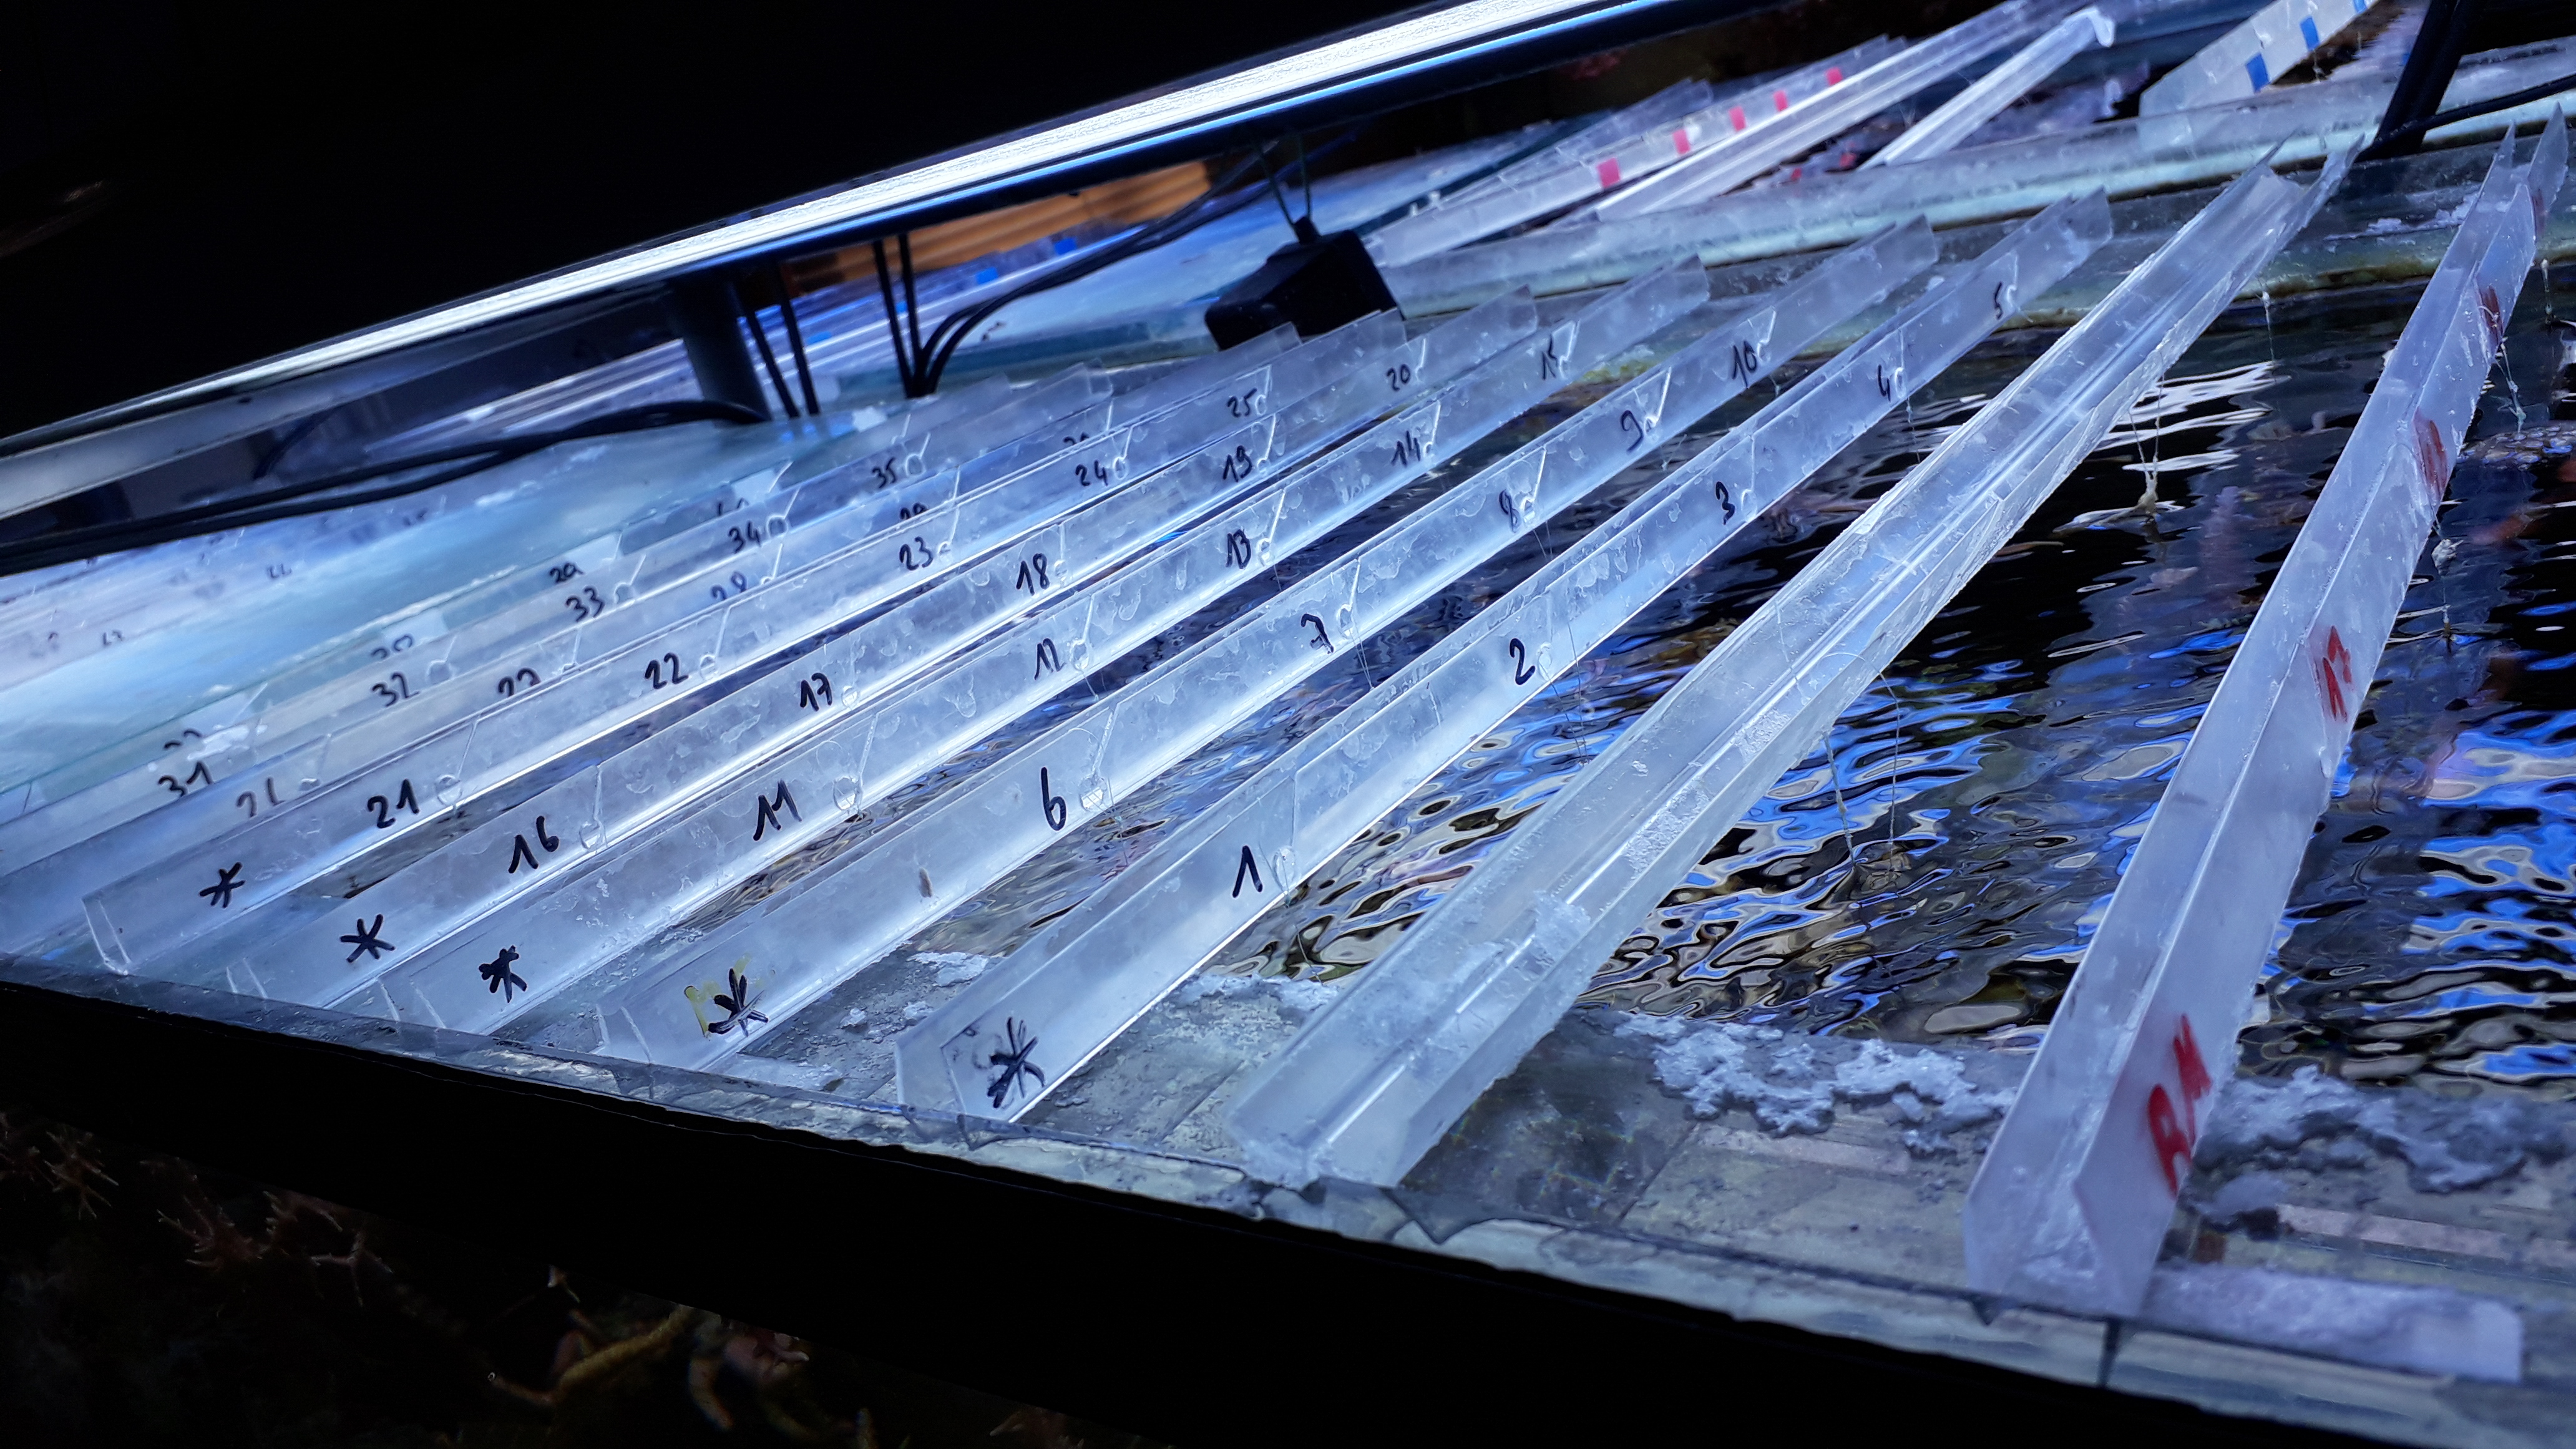
\includegraphics[]{../image/regle.jpg}
\caption{Règle numérotée}
\end{figure}

\begin{figure}[h!]
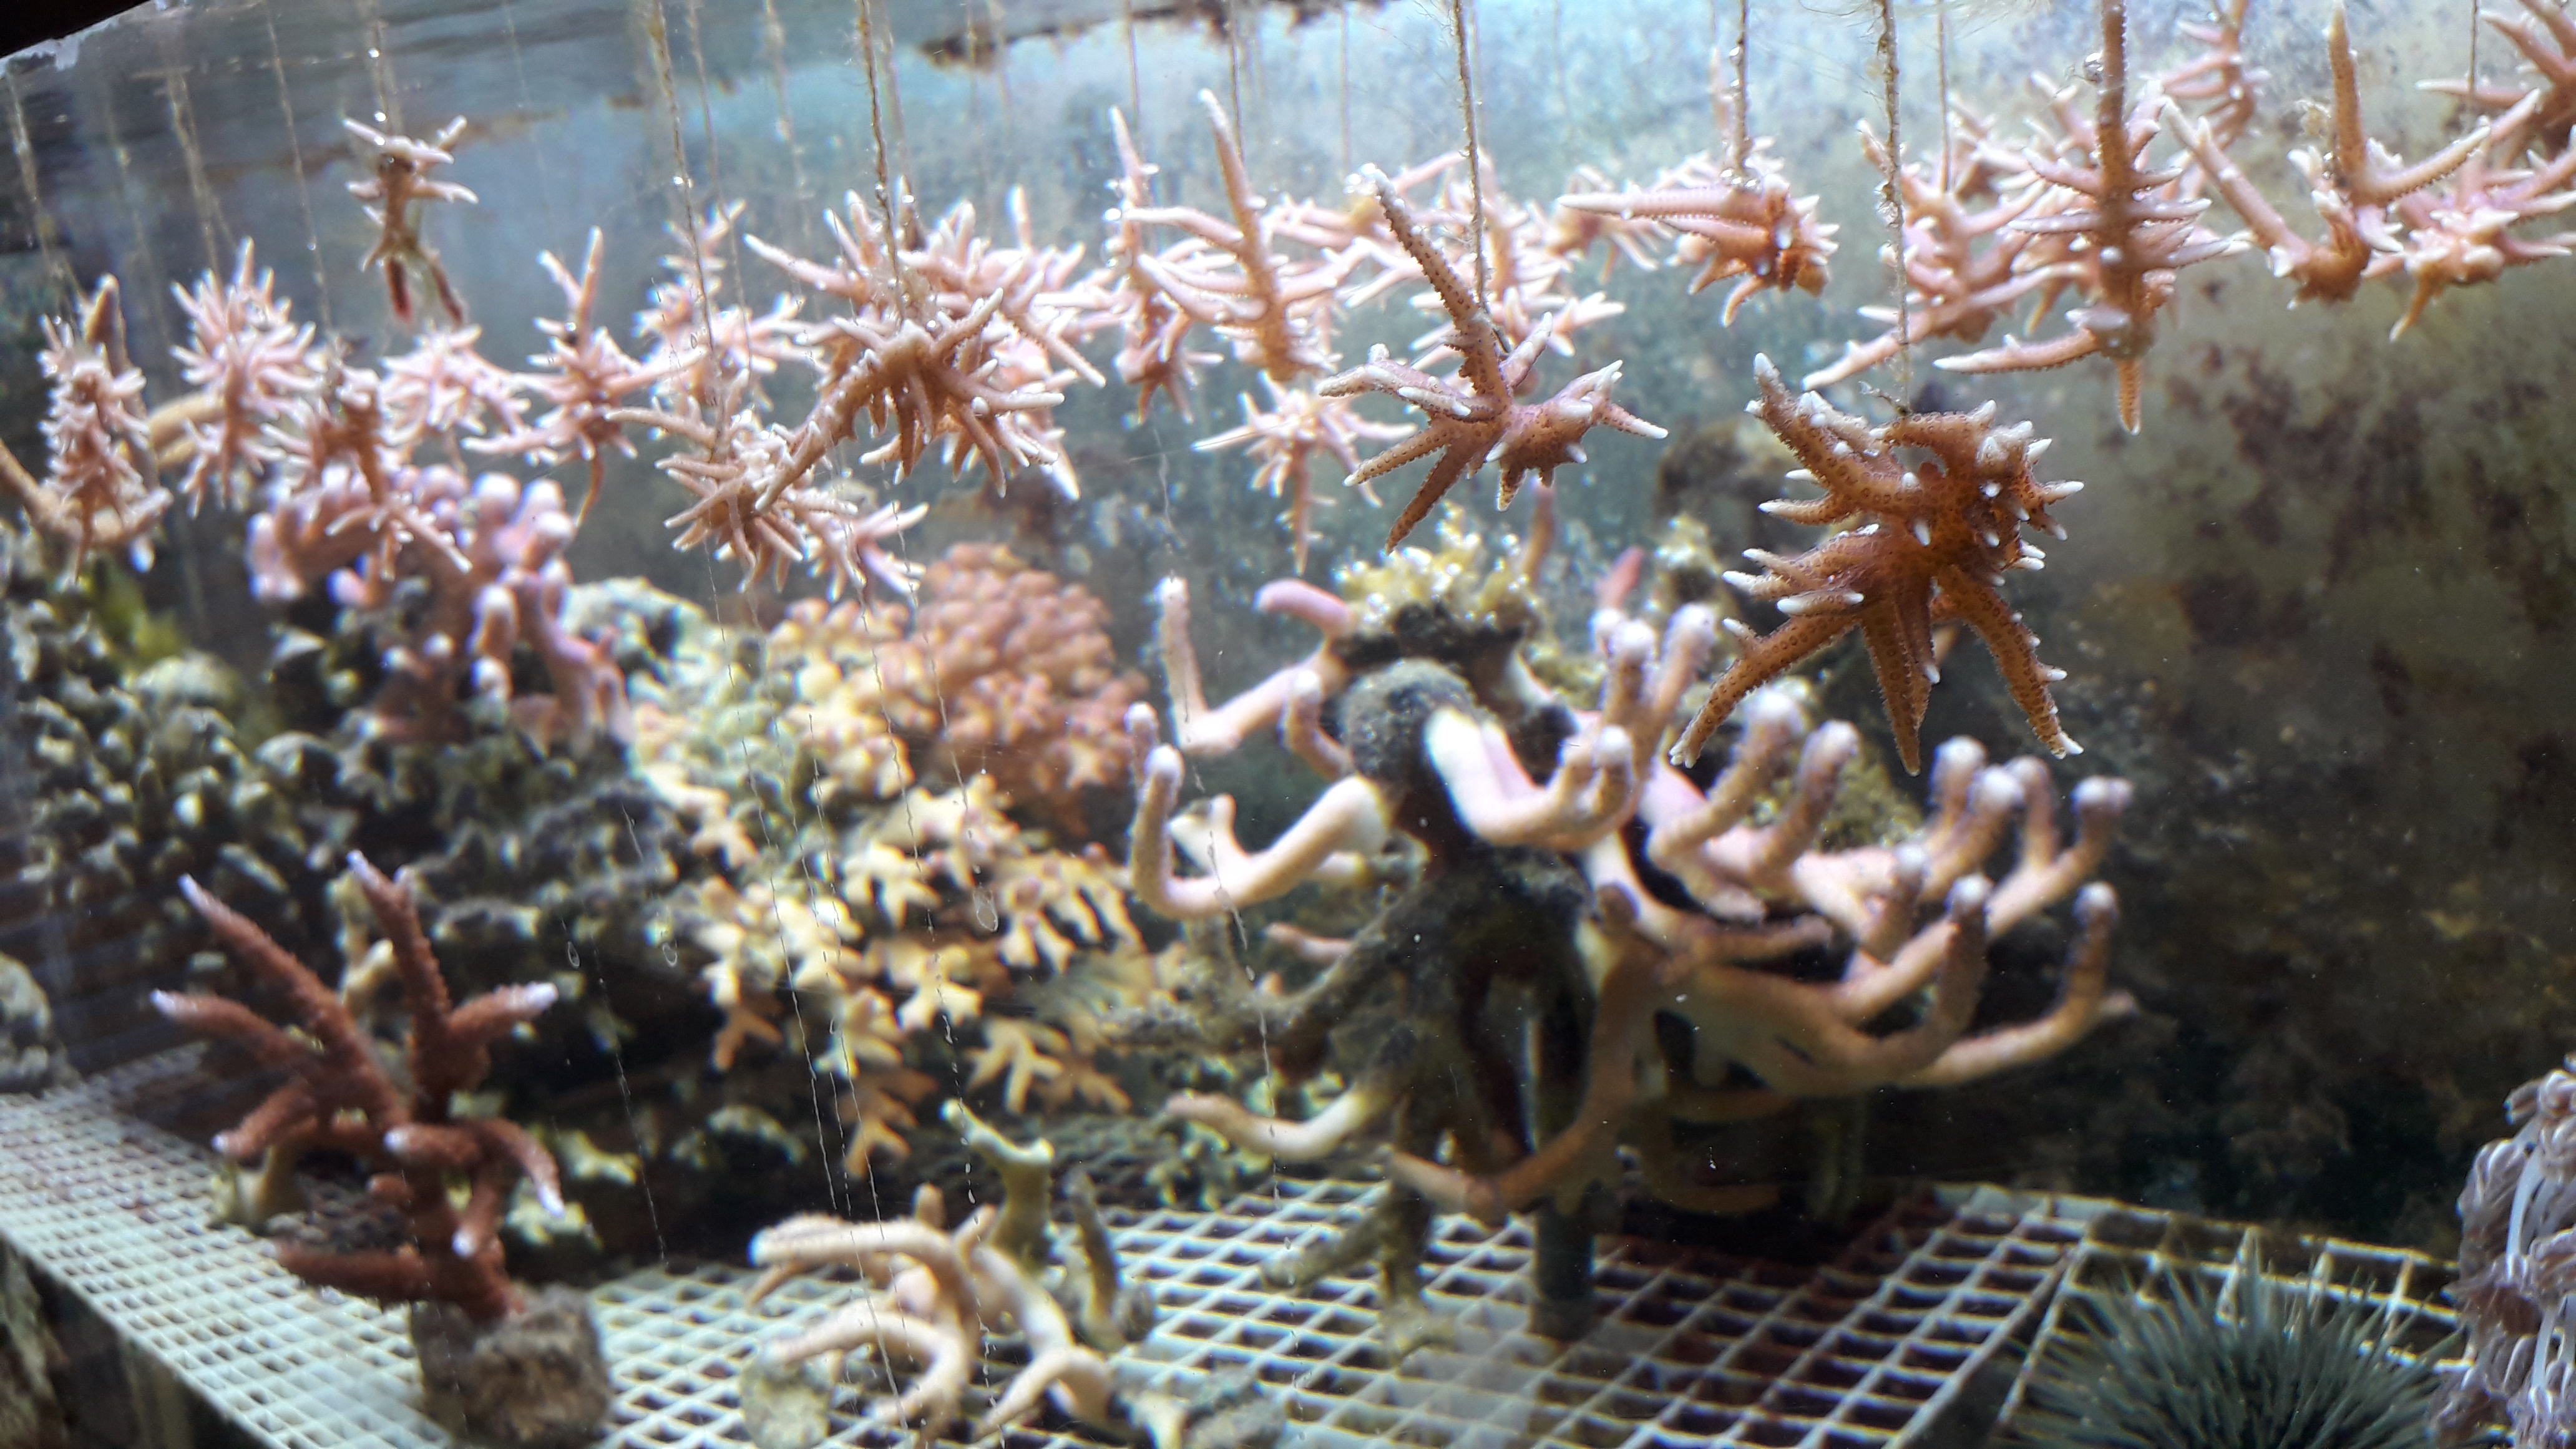
\includegraphics[]{../image/boutures.jpg}
\caption{Boutures suspendues de *Seriatopora hystrix*}
\end{figure}

\subsection{Outils monitorings}\label{outils-monitorings}

\subsubsection{Masse immergée et masse
squelettique}\label{masse-immergee-et-masse-squelettique}

Pour évaluer la croissance des boutures de coraux, on utilise la masse
squelettique. Pour l'obtenir sans détruire le corail, on mesure la masse
immergée du corail dans l'eau de mer avec une balance munie d'un crochet
(Fig. 4.3). Cette méthode de mesure est rapide et peu stressante pour
les organismes. Après avoir mesuré la température et la salinité, on
peut convertir la masse immergée en masse squelettique à l'aide de la
formule ci-dessous mise au point par Jokiel \emph{et al} (1978) :

\begin{equation}
\large
  m_{squelettique} = \frac {m_{immerge}}{ 1 - \frac{\rho_{eau}}{ \rho_{squelettique}}}
\end{equation}

\(\rho_{eau}\) est déterminé par l'équation d'état de l'eau de mer grâce
à la mesure de la salinité et de la température. Le
\(\rho_{squelettique}\) est la densité de l'aragonite
(CaCO\textsubscript{3}) du squelette du corail.

\begin{centering}
\begin{figure}[h!]
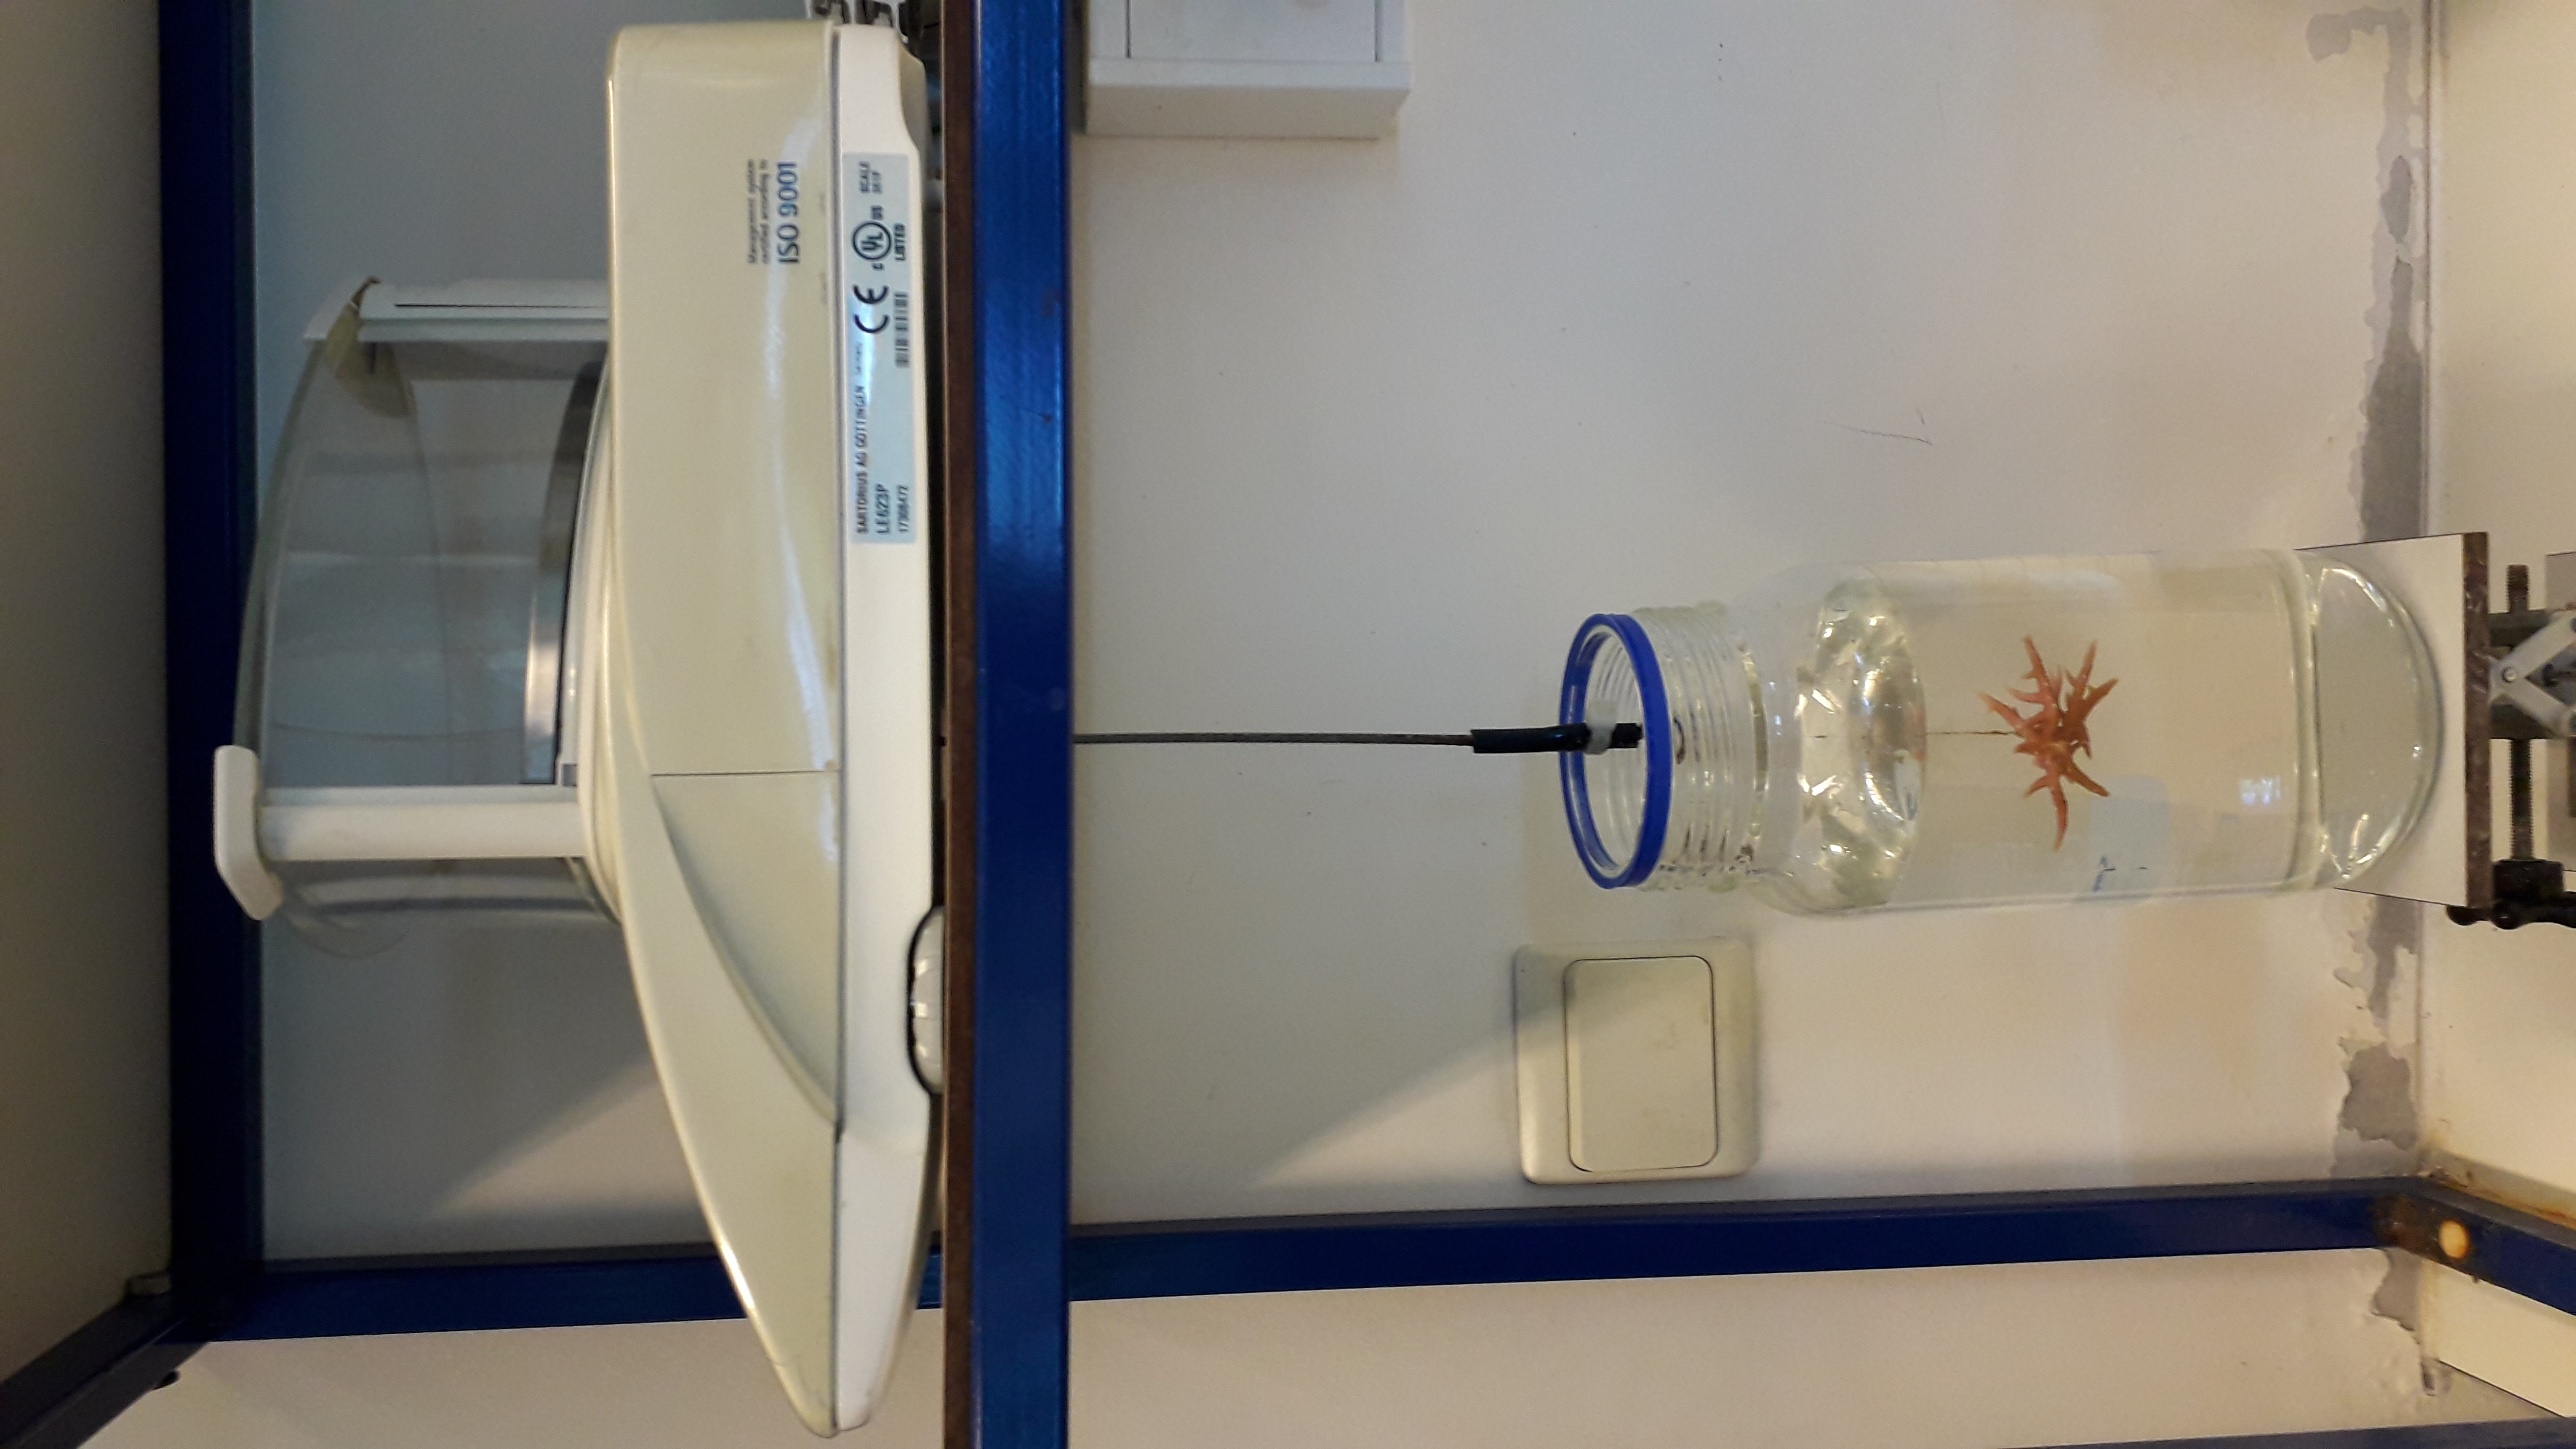
\includegraphics[angle=270]{../image/poster-balance.jpg}
\caption{Mesure du poids immergé d'une bouture}
\end{figure}
\end {centering}

\subsubsection{Tableur en ligne}\label{tableur-en-ligne}

Les mesures effectuées sur les coraux et les paramètres de l'eau des
mésocosmes sont dans un premier temps notés dans un cahier de
laboratoire. Il sera nécessaire de créer un nouveau tableau de donnée
afin d'utiliser les données.

Au début, le tableur choisi était Excel, car c'est le logiciel le plus
connu et que la HEH me permet d'utiliser une licence. Cela fonctionnait
bien avec les fichiers en local. Malheureusement, aucun package ne
permet d'utiliser Excel en ligne.

C'est avec Googlesheets qu'une solution fut trouvée.

Le tableur est en ligne cela permet à n'importe quelle personne de
manipuler le tableau de données depuis n'importe quelle machine
connectée à internet.

Afin d'éviter au maximum des erreurs d'encodages, des règles de mise en
forme conditionnelles ont été créées pour mettre en évidence les cases
non remplies, formater le type des cellules et mettre un dégradé de
couleur suivant l'avancement des données (Fig. 4.4).

\begin{figure}[h!]
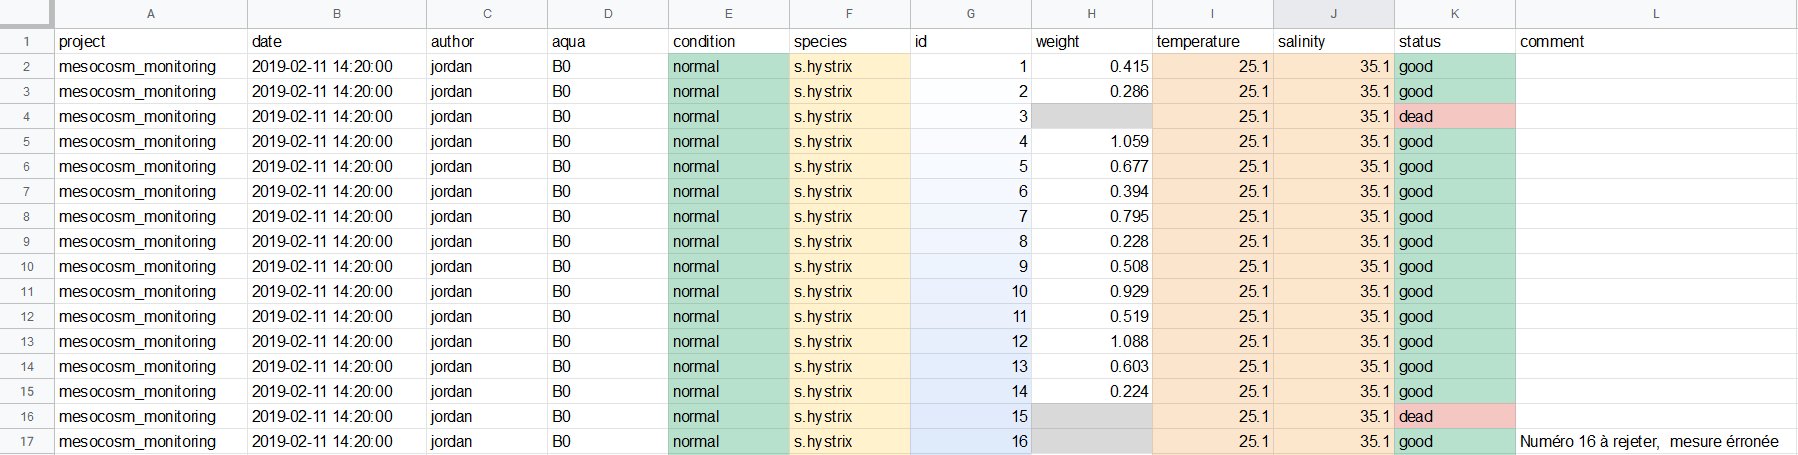
\includegraphics[]{../image/tableur-gs.PNG}
\caption{Tableur en ligne Google Sheets}
\end{figure}

Le tableur est divisé en 12 colonnes :

\begin{itemize}
\tightlist
\item
  project : différencie chaque expérience réalisée, généralement on
  préfèrera recréer un nouveau tableur pour chacune des expériences
\item
  date : date et heure à laquelle les relevés de mesures ont été pris
\item
  author : nom de la personne ayant encodé dans le tableur
\item
  aqua : nom du mésocosme où la bouture a été prélevé
\item
  condition : condition spécifique appliquée à la bouture (exemple :
  stress hypersalin)
\item
  species : nom de l'espèce mesurée
\item
  id : numéro de la bouture mesurée
\item
  weight : masse immergée mesurée
\item
  temperature : température de l'eau de mer
\item
  salinity : salinité de l'eau de mer
\item
  status : état de santé de la bouture
\item
  comment : commentaire
\end{itemize}

\subsection{Présentation de l'application
Shiny}\label{presentation-de-lapplication-shiny}

L'application est divisée en deux fichiers, une partie ``ui'' (User
Interface), c'est la partie qui affiche les éléments graphiques de
l'interface Shiny à l'utilisateur et une partie ``server'', qui contient
toutes les commandes R qui s'opère côté serveur.

Il est possible mettre l'intégralité du code dans un seul fichier app.R.
Cependant, j'ai divisé mon script en deux fichiers ui.R et server.R pour
plus de clarté (voir partie annexe).

\vspace{1 cm}

Mon application présente 3 onglets, le premier créer un graphique
interactif (Fig. 4.5).

\begin{figure}[h!]
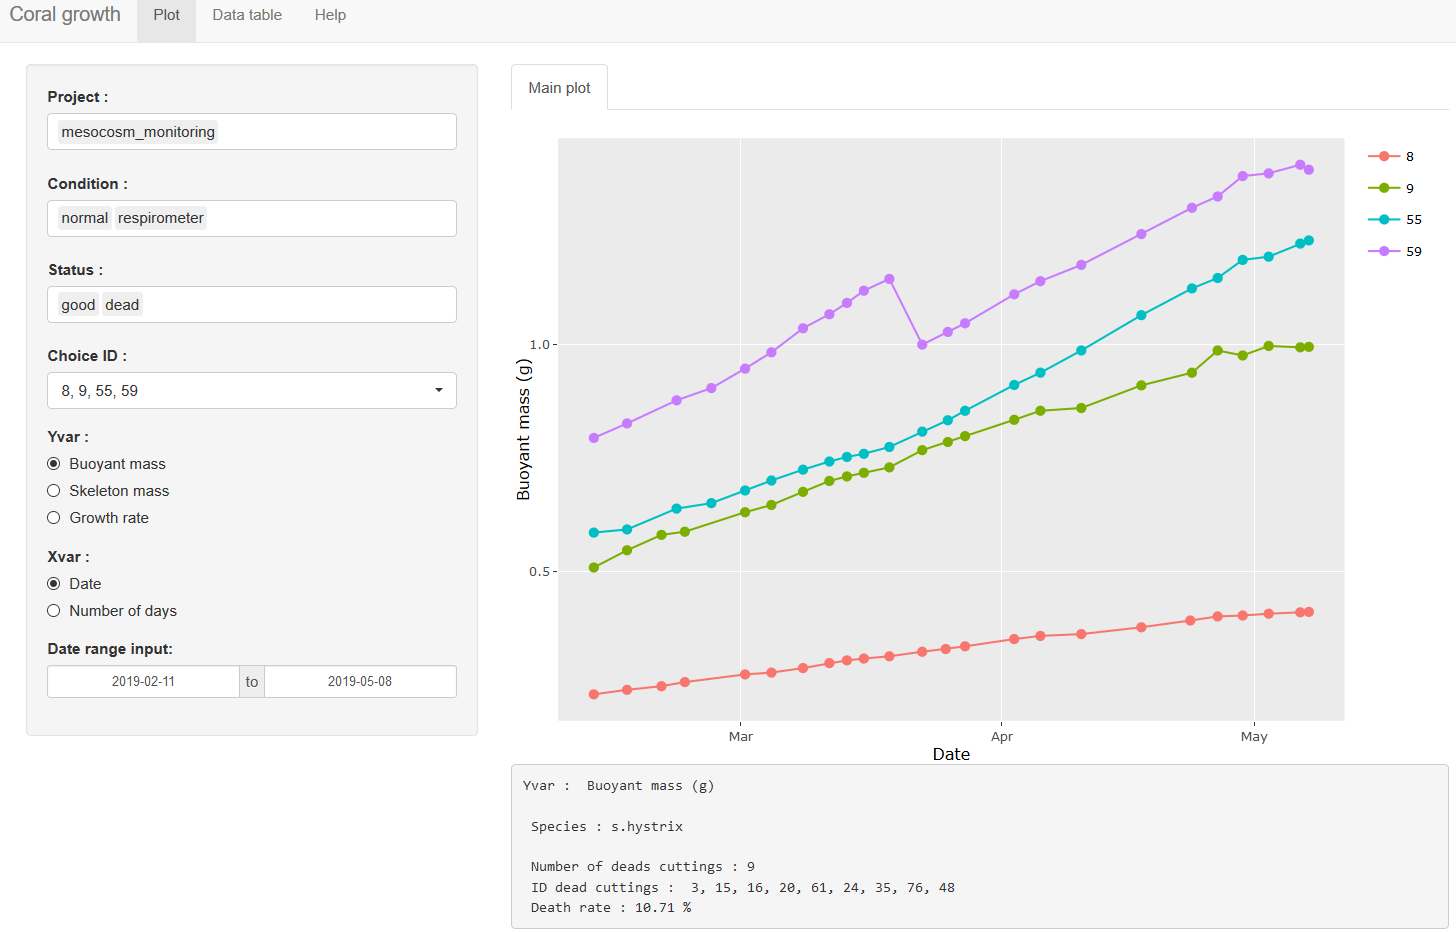
\includegraphics[]{../image/notebook-plot1.PNG}
\caption{Application Shiny : onglet "Plot"}
\end{figure}

\vspace{0.5 cm}

Par défaut, le graphique utilise en ordonnée la masse immergée des
boutures et en abscisse la date de la mesure. Les boutures sélectionnées
sont peu nombreuses pour l'exemple, mais il est possible de toutes les
sélectionner.

\vspace{0.5 cm}

Différents paramètres peuvent modifier le graphique (Fig. 4.6).

\begin{figure}
\centering
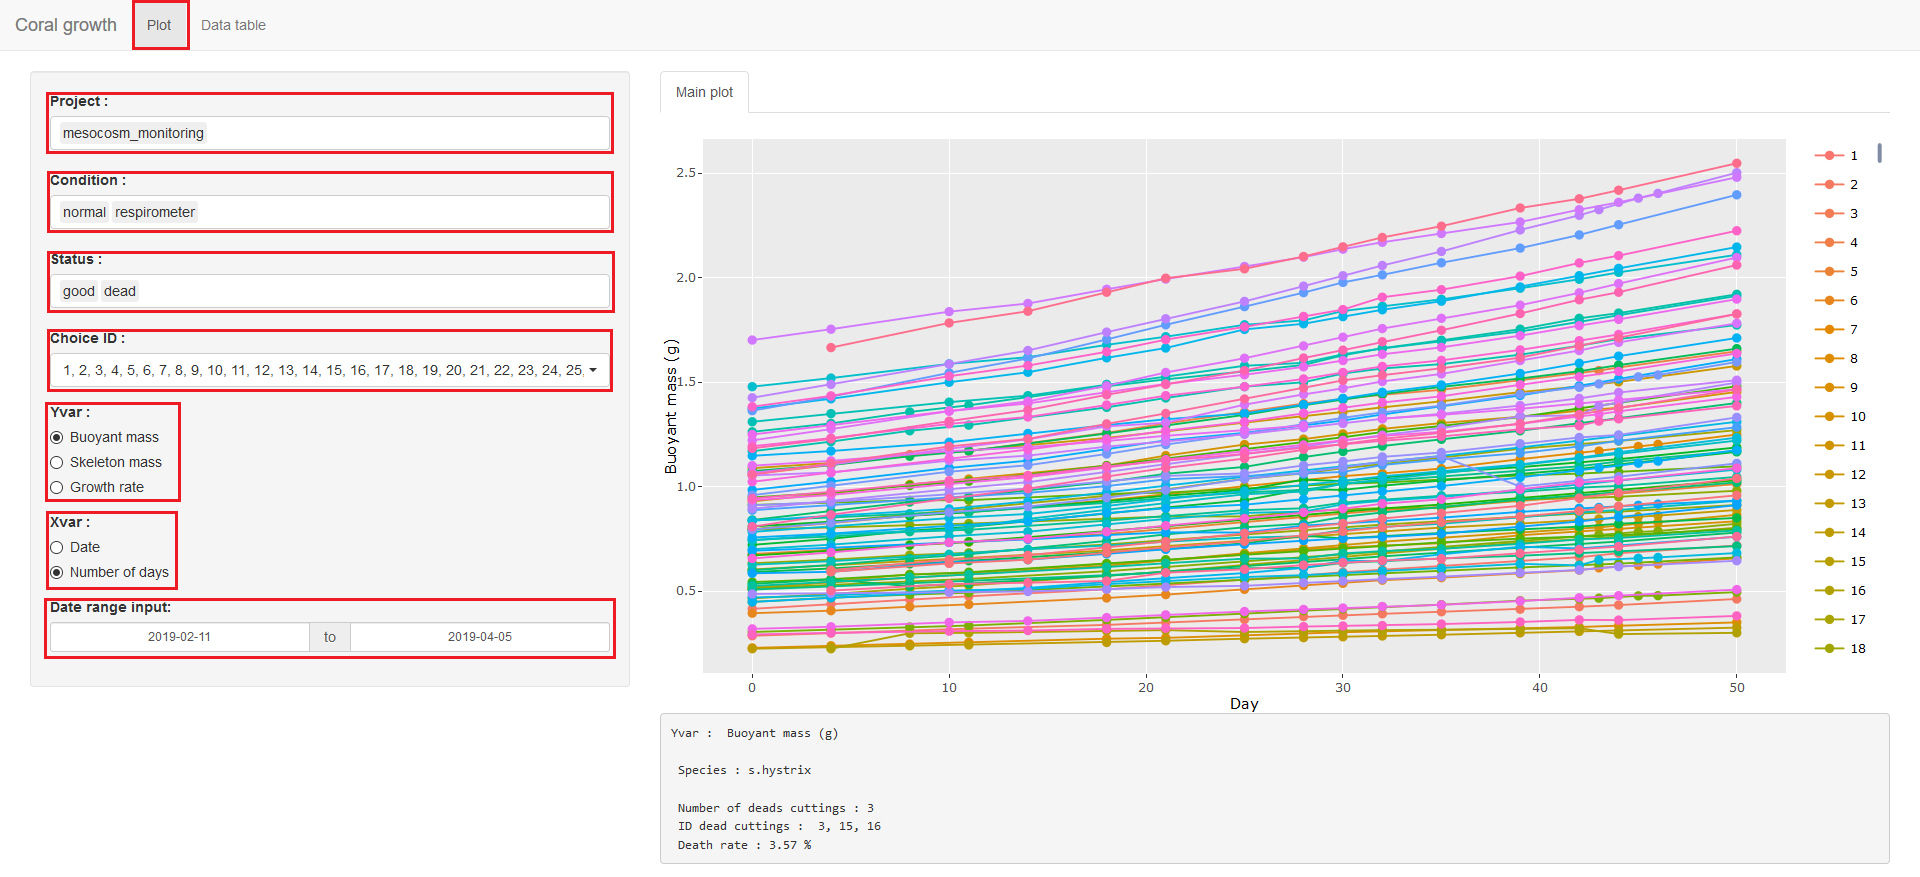
\includegraphics[width=15.00000cm]{../image/notebook-plot2.PNG}
\caption{Application Shiny : paramètres}
\end{figure}

\vspace{0.5cm}

En ordonnée, on peut choisir :

\begin{itemize}
\tightlist
\item
  la masse immergée
\item
  la masse squelettique
\item
  le taux de croissance (Fig. 4.7) 
\end{itemize}

\begin{figure}[h!]
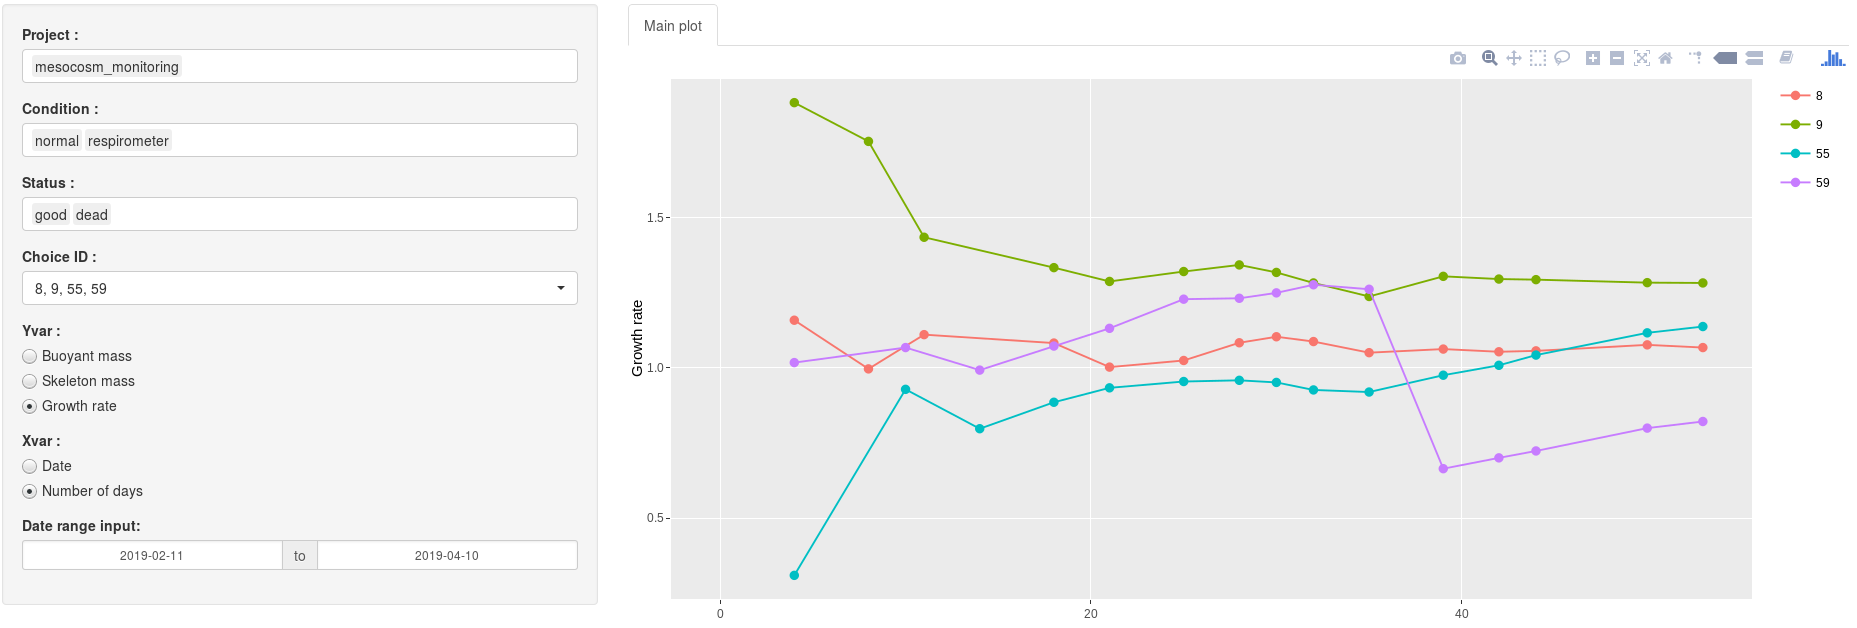
\includegraphics[]{../image/taux-croissance.PNG}
\caption{Application Shiny : taux de croissance}
\end{figure}

En abscisse, on peut choisir :

\begin{itemize}
\tightlist
\item
  la date de la mesure
\item
  le nombre de jours écoulés depuis la première mesure
\end{itemize}

Il est également possible de restreindre la période de temps (option
\emph{Date range input}).

Il est aussi possible de sélectionner les ID dans un menu déroulant, on
peut également désélectionner les lignes en cliquant sur le numéro
associer à la couleur de l'ID à droite de l'écran (Fig. 4.8, Fig. 4.9).

La fenêtre du menu déroulant a maintenant une taille adaptée et ne
dépasse pas du cadre. Il permet de sélectionner ou de désélectionner
toutes les boutures en deux cliques ou de sélectionner/désélectionner
les boutures unes à unes.

\begin{figure}[h!]
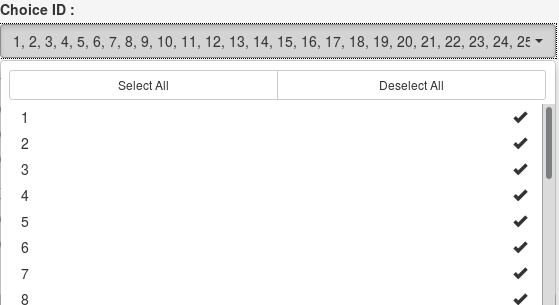
\includegraphics[]{../image/menu-deroulant.PNG}
\caption{Application Shiny : menu déroulant}
\end{figure}

En passant le curseur sur les points du graphique, on peut obtenir
quelques informations supplémentaires (Fig. 4.10).

\begin{figure}[h!]
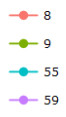
\includegraphics[]{../image/shiny-selection.PNG}
\caption{Application Shiny : affichage intéractif}
\end{figure}

\begin{figure}[h!]
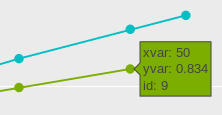
\includegraphics[]{../image/info-curseur.PNG}
\caption{Application Shiny : information via le curseur}
\end{figure}

En bas du graphique, des informations supplémentaires sont données (Fig.
4.11) :

\begin{itemize}
\tightlist
\item
  Yvar : l'ordonnée du graphique
\item
  Species : l'espèce des boutures
\item
  Number of deads cuttings : le nombre de boutures mortes
\item
  ID dead cuttings : l'ID des boutures mortes
\item
  Death rate : le taux de mortalité
\end{itemize}

\begin{figure}[h!]
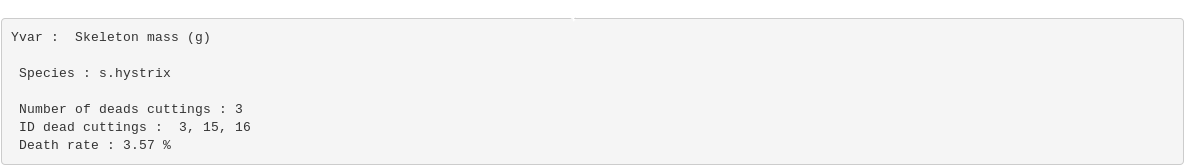
\includegraphics[]{../image/verbatim.PNG}
\caption{Application Shiny : informations supplémentaires}
\end{figure}

Le deuxième onglet contient le tableau de donnée où de nouvelles
colonnes ont été calculées, il y a l'ajout de la masse squelettique et
du ``ratio'' qui correspond au taux de croissance (Fig. 4.12).

\begin{figure}[h!]
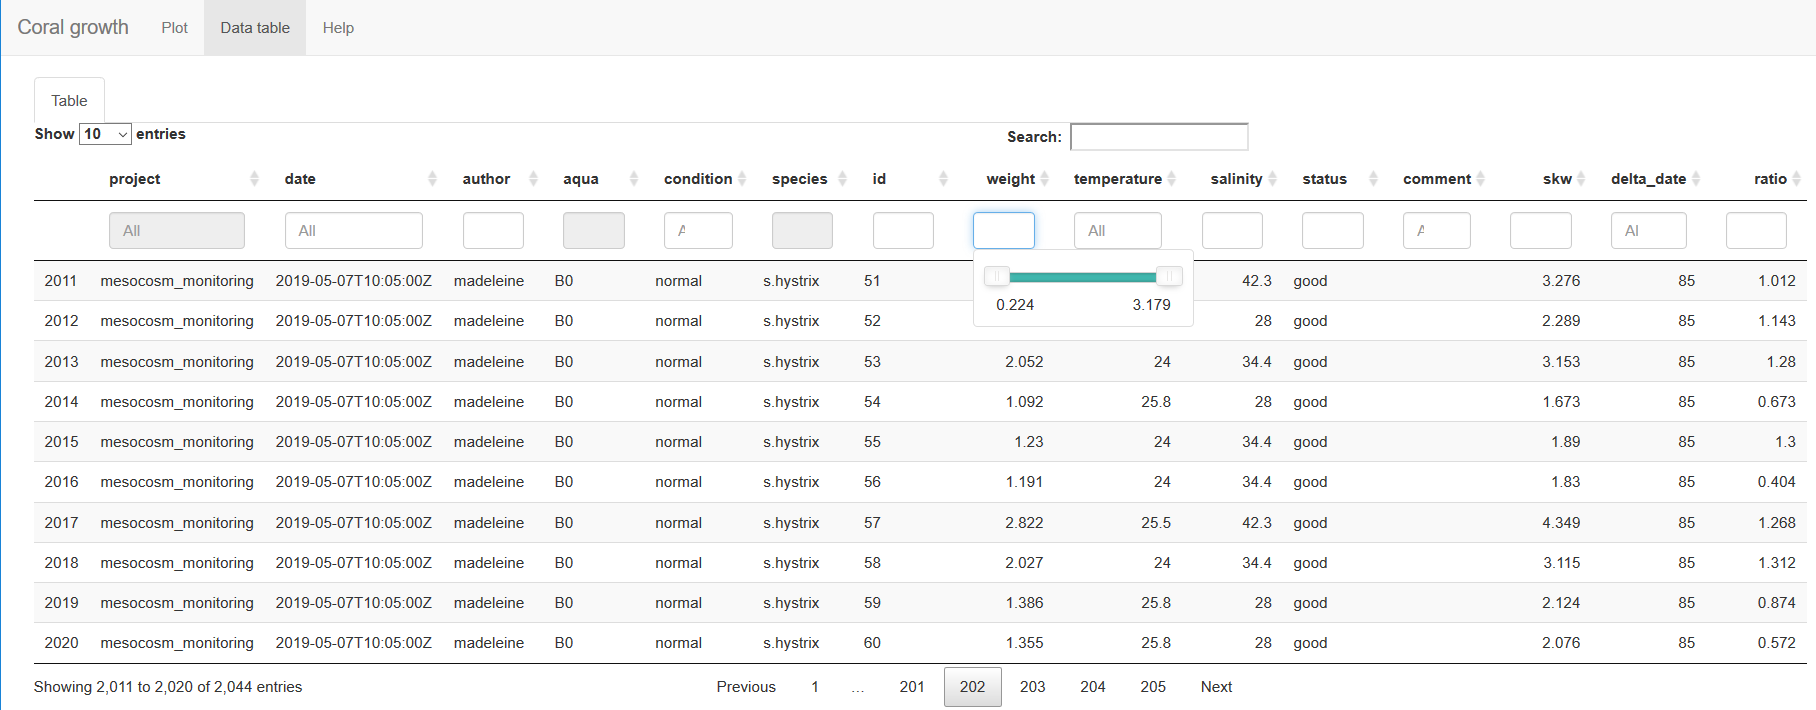
\includegraphics[]{../image/notebook-table1.png}
\caption{Application Shiny : tableau de donnée}
\end{figure}

Le dernier onglet contient une page d'aide (Fig. 4.13). Cette
documentation permettra aux utilisateurs de comprendre comment utiliser
l'application et permettra aussi de comprendre comment fonctionne le
code. Il est important de documenter son travail si l'on veut qu'il
puisse être réutilisé par la suite.

\begin{figure}[h!]
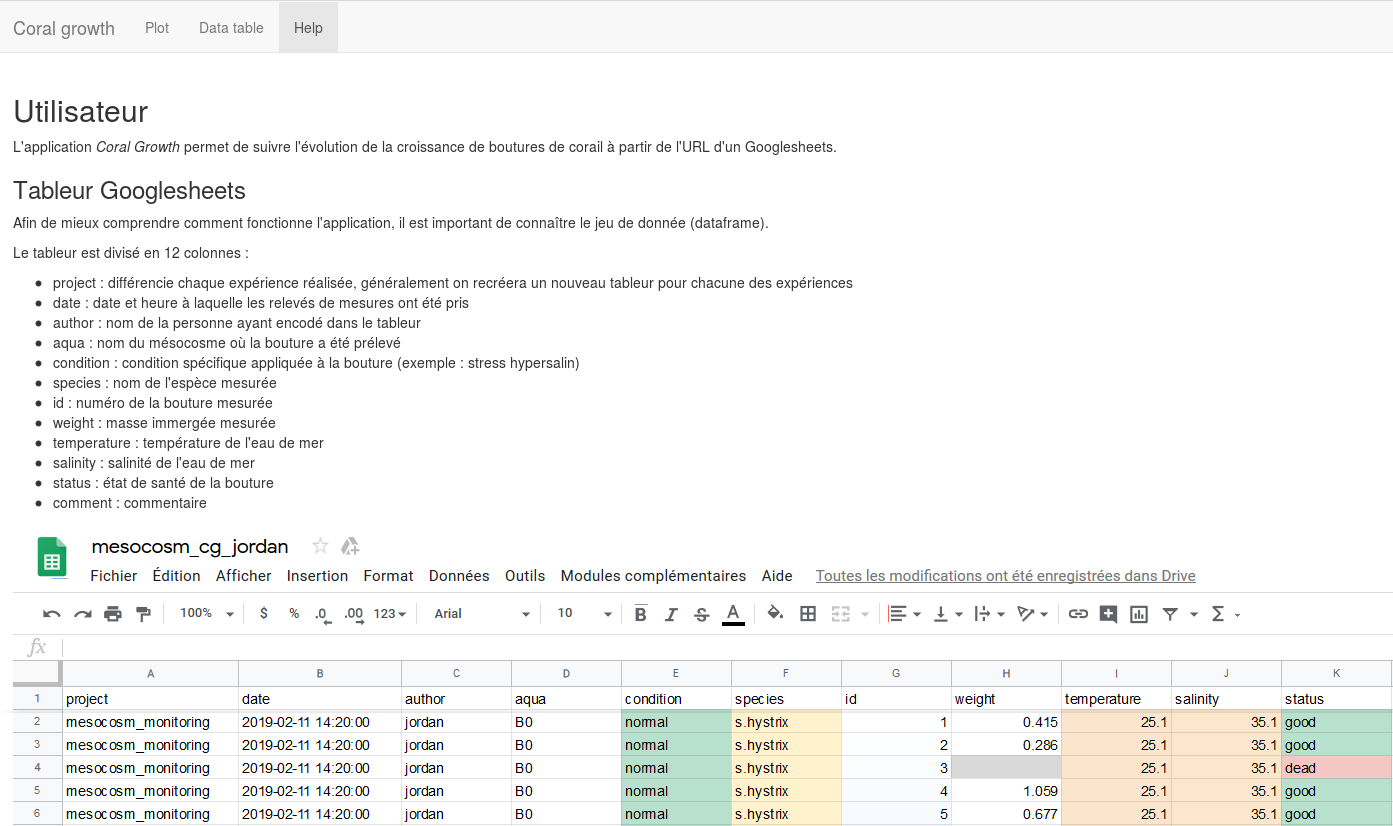
\includegraphics[]{../image/aide.PNG}
\caption{Application Shiny : onglet aide}
\end{figure}

\subsection{Difficultés rencontrées}\label{difficultes-rencontrees}

\subsubsection{R vs python}\label{r-vs-python}

La principale difficulté rencontrée au début est de passer de
l'apprentissage du langage de programmation \emph{python} à \emph{R}. Ce
sont tous les deux des langages de programmation interprétés qui peuvent
être utilisés dans le domaine du traitement de donnée et de création
d'application web. \emph{python} a été créé pour faire de la
programmation informatique généraliste, il est utilisé dans de larges
domaines par des informaticiens. A l'inverse, R est dédié aux analyses
statistiques, plutôt utilisées par des spécialistes ou des
scientifiques.

Dans le domaine du \emph{data scientist}, \emph{R} et \emph{python} sont
couramment employé.

\subsubsection{Shiny communication entre ui.R et
server.R}\label{shiny-communication-entre-ui.r-et-server.r}

Les applications web gérées par shiny utilisent deux fonctions
communiquant entre elles \textbf{ui} et le \textbf{server}.

Le schéma de communication basique entre les deux scripts commence par
la déclaration d'une variable \emph{inputId = ma\_variable} dans ui.R.
Celui-ci est appelé dans server.R sous la forme
\emph{input\$ma\_variable}, cette variable sera ensuite traitée dans un
bloc de code délimiter par des crochets.

Shiny utilise du Javascript pour dynamiser l'interface de l'utilisateur
sous une couche de code masqué, cette couche simplifie grandement le
travail avec R. Si on sort du cadre de l'utilisation prévu par Shiny, on
se heurte à de grands soucis de codage. Shiny restreint donc, la
communication entre les différents blocs de code. Dans certaines
situations cela complique le travail, ce fut notamment le cas lors de la
création du menu déroulant qui a besoin de connaître dans ui.R le nombre
d'ID qui est nécessaire, sauf que la variable donnant cette information
est dans server.R et Shiny permet difficilement de faire cela.

\subsection{Objectifs réalisés}\label{objectifs-realises}

Les objectifs réalisés sont :

\begin{itemize}
\item
  Apprendre les bases du langage R et différents packages R.
\item
  Maîtriser l'outil RStudio.
\item
  Bouturer les coraux et relever leurs masses immergées.
\item
  Créer un tableau de données en ligne contenant les données
  nécessaires.
\item
  Créer une application web exploitant en continue les données du
  tableau en ligne.
\item
  Réaliser un code simple et documenté.
\item
  Utiliser le service web Github afin de réaliser un travail
  professionnel.
\end{itemize}

L'outil insight de Github permet de visualiser le travail des différents
contributeurs sur un même projet. On peut constater le travail réalisé
pendant le stage (Fig. 4.14).

\begin{figure}
\centering
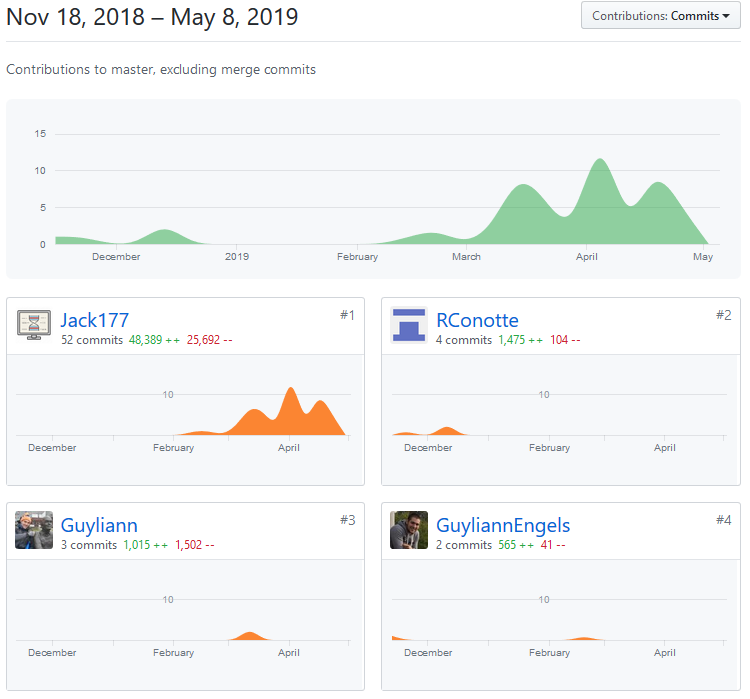
\includegraphics{../image/github.PNG}
\caption{Contributeur de l'application}
\end{figure}

\section{Conclusion}\label{conclusion}

Le point de départ de ce stage est l'application précédente effectuée
par Raphaël Conotte. Pour comprendre son travail, il a fallu dans un
premier temps apprendre le langage de programmation R et ses composants.
Deuxièmement, il a fallu lire et comprendre son code ainsi que le jeu de
données qu'il a utilisé. Dans le même temps, j'ai appris à multiplier du
corail, les peser et créer mon propre jeu de données.

On m'a donné la possibilité de soit repartir du code précédent, soit de
tout réécrire. C'est le second choix que j'ai pris, car le code de
Raphaël étant encore aujourd'hui toujours trop complexe à mes yeux, je
pense qu'il a voulu tester différentes manières de faire.

Le début de mon code était donc un fichier vide que j'ai rempli au fur
et à mesure, en m'inspirant parfois du code de Raphaël. Je pense avoir
rendu un code beaucoup plus simple à lire et mieux documenté.
L'application que j'ai réalisée se démarque de celle de Raphaël. En plus
de trier la base de données par projet, elle permet également de
combiner les tris par condition et par l'état des boutures.

Contrairement à l'application précédente qui ne contenait que 6
boutures, mon travail en compte 84. Dans le but de faciliter la
sélection de celles-ci, le menu déroulant a été perfectionné.

Le tableau de données présenté dans l'onglet ``Data table'' a été
simplifié, mais il permet de faire un tri sur chacune des colonnes à
l'aide d'un curseur de déplacement ``slider''.

L'application est actuellement en ligne et est disponible à l'adresse
suivante : \url{https://jack177.shinyapps.io/coralgrowth/}

Une documentation au format \emph{bookdown} a été écrite pour les
utilisateurs du laboratoire, mais aussi pour l'informaticien qui
souhaiterait améliorer le code. En effet, le travail peut-être amélioré.
On pourrait ajouter plusieurs jeux de données à partir d'une url,
ajouter des visualisations différentes afin de permettre un autre point
vue sur le jeu de donnés ou encore de placer mon code dans un package
afin d'être utilisé par n'importe qui utilisant R.

Le dernier onglet ``Help'' contient la documentation bookdown et le
dépôt Github où se trouve la dernière version du code utilisée.

Il est également possible de scanner le \emph{QR code} (Fig. 4.15) qui
redirige vers l'application.

\begin{figure}[h!]
\begin{centering}

\includegraphics[width=6cm]{../image/QRcode.png}
\caption{QR code}
\end{centering}
\end{figure}

D'un point de vue personnel, ce stage m'a permis de m'insérer dans une
petite équipe où je me suis rapidement intégré. J'ai pu fréquenter un
laboratoire de recherche et en apprendre beaucoup sur la vie marine et
le milieu universitaire.

Le travail que j'ai effectué était passionnant. Je me suis rendu compte
des différentes possibilités que peut offrir l'informatique à la
biologie ainsi que la valeur ajoutée que j'ai pu proposer.

J'ai travaillé comme un professionnel sur un projet que j'ai vu se
réaliser petit à petit, en utilisant des outils propres aux
informaticiens comme Github. J'ai acquis des connaissances sur le
traitement de données, découvert le langage de programmation \emph{R} et
appris a rédiger en \emph{LaTeX}/\emph{R Markdown} ce rapport.

Je souhaiterai poursuivre das cette voie en apprenant à traiter des
données avec \emph{python} à l'aide des paquets \emph{Numpy} et
\emph{Pandas} afin de le comparer à R et également apprendre le langage
\emph{javascript} utilisé par le package \emph{shiny} qui rend les pages
web dynamiques.


\end{document}
